\section{Beispielrechnung eines Fahrtverlaufs im \ac{ebuef}} \label{beispielrechnungKapitel}
Die in Kapitel \ref{kapitelFahrtverlauf} beschriebene Berechnung des Fahrtverlaufs wird in diesem Kapitel an einer Beispielfahrt von Ausblick (XAB) nach Zoo (XZO) exemplarisch gezeigt. Dafür wurde dem Zug ein Fahrplan zugewiesen, nach dem der Zug nach \Gls{simulationszeit} um 10:00:05 in Ausblick losfahren soll und um 10:02:00 in dem Bahnhof Zoo ankommen soll. Zu Beginn steht der Zug im \ac{infra} 1189 (XAB), hat die Fahrtrichtung 1 und die \Gls{fahrstrasse} ist so eingestellt, dass das Fahrzeug bis zum Ausfahrsignal im Bahnhof Zoo fahren kann und dort im \ac{infra} 1178 zum Stehen kommen kann. Somit beträgt die Strecke bis zum nächsten Halt 672 $m$ und das Fahrzeug hat 115 $s$ zur Verfügung. Die Bremsverzögerung des Fahrzeugs beträgt 0,8 $m/s^{2}$.

Für die Fahrt wurde eine Mindestzeit von 20 $s$ für \Gls{beharrungsfahrt}en (\textit{\$glo\-bal\-Time\-On\-One\-Speed = 20}) festgelegt, den Optionen \textit{\$useSpeedFineTuning}, \textit{\$useMinTimeOnSpeed} und \textit{\$slowDownIfTooEarly} wurde der Wert \textit{true} zugewiesen und der Option \textit{\$errorMinTimeOnSpeed} der Wert \textit{false}.

In der Tabelle \ref{table:beispielebuefkeypoint} sind die berechneten \textit{\$keyPoints} aufgelistet, welche durch die Berechnung des Fahrtverlaufs ermittelt wurden, und in der Darstellung \ref{fig:it14} ist der Fahrtverlauf visuell dargestellt. Bei der Berechnung des \Gls{fahrtverlauf}s wurde laut der Fahrzeugsteuerung die Ankunftszeit exakt eingehalten. Die Zeit-Werte der \textit{\$keyPoints} geben bei der Berechnung die \Gls{simulationszeit} im Unix-Timestamp-Format an und sind deswegen ebenfalls im Format \textit{hh:mm:ss} angegeben.
\begin{table}
\begin{center}
\renewcommand{\arraystretch}{1.2}
\begin{tabular}{c|c|c|c}
\textit{\$keyPoint}-Index & 0 & 1 & 2 \\ \hline
\textit{\$speed\_0}                   &   0 $km/h$    & 30 $km/h$ & 10 $km/h$                     \\ \hline
\textit{\$speed\_1}                &       30 $km/h$& 10 $km/h$ & 0 $km/h$             \\ \hline
\textit{\$position\_0}                  &   0 $m$    & 528.83 $m$ & 667.18 $m$                   \\ \hline
\textit{\$position\_1}                 &       43.40 $m$ & 567.41 $m$ & 672 $m$        \\ \hline
\textit{\$time\_0} (Unix-Timestamp)                 &   1631088005    & 1631088073,67 & 1631088116,53             \\ \hline
\textit{\$time\_1} (Unix-Timestamp)             &       1631088015,41& 1631088080,61 & 1631088120           \\ \hline
\textit{\$time\_0} (hh:mm:ss)                   &   10:00:05    & 10:01:14 & 10:01:57             \\ \hline
\textit{\$time\_1} (hh:mm:ss)               &       10:00:15& 10:01:21 & 10:02:00           \\ 
\end{tabular}
\renewcommand{\arraystretch}{1}
\caption{\textit{\$keyPoints} am Beispiel von der Fahrt von XAB nach XZO}
\label{table:beispielebuefkeypoint}
\end{center}
\end{table}
\begin{figure}
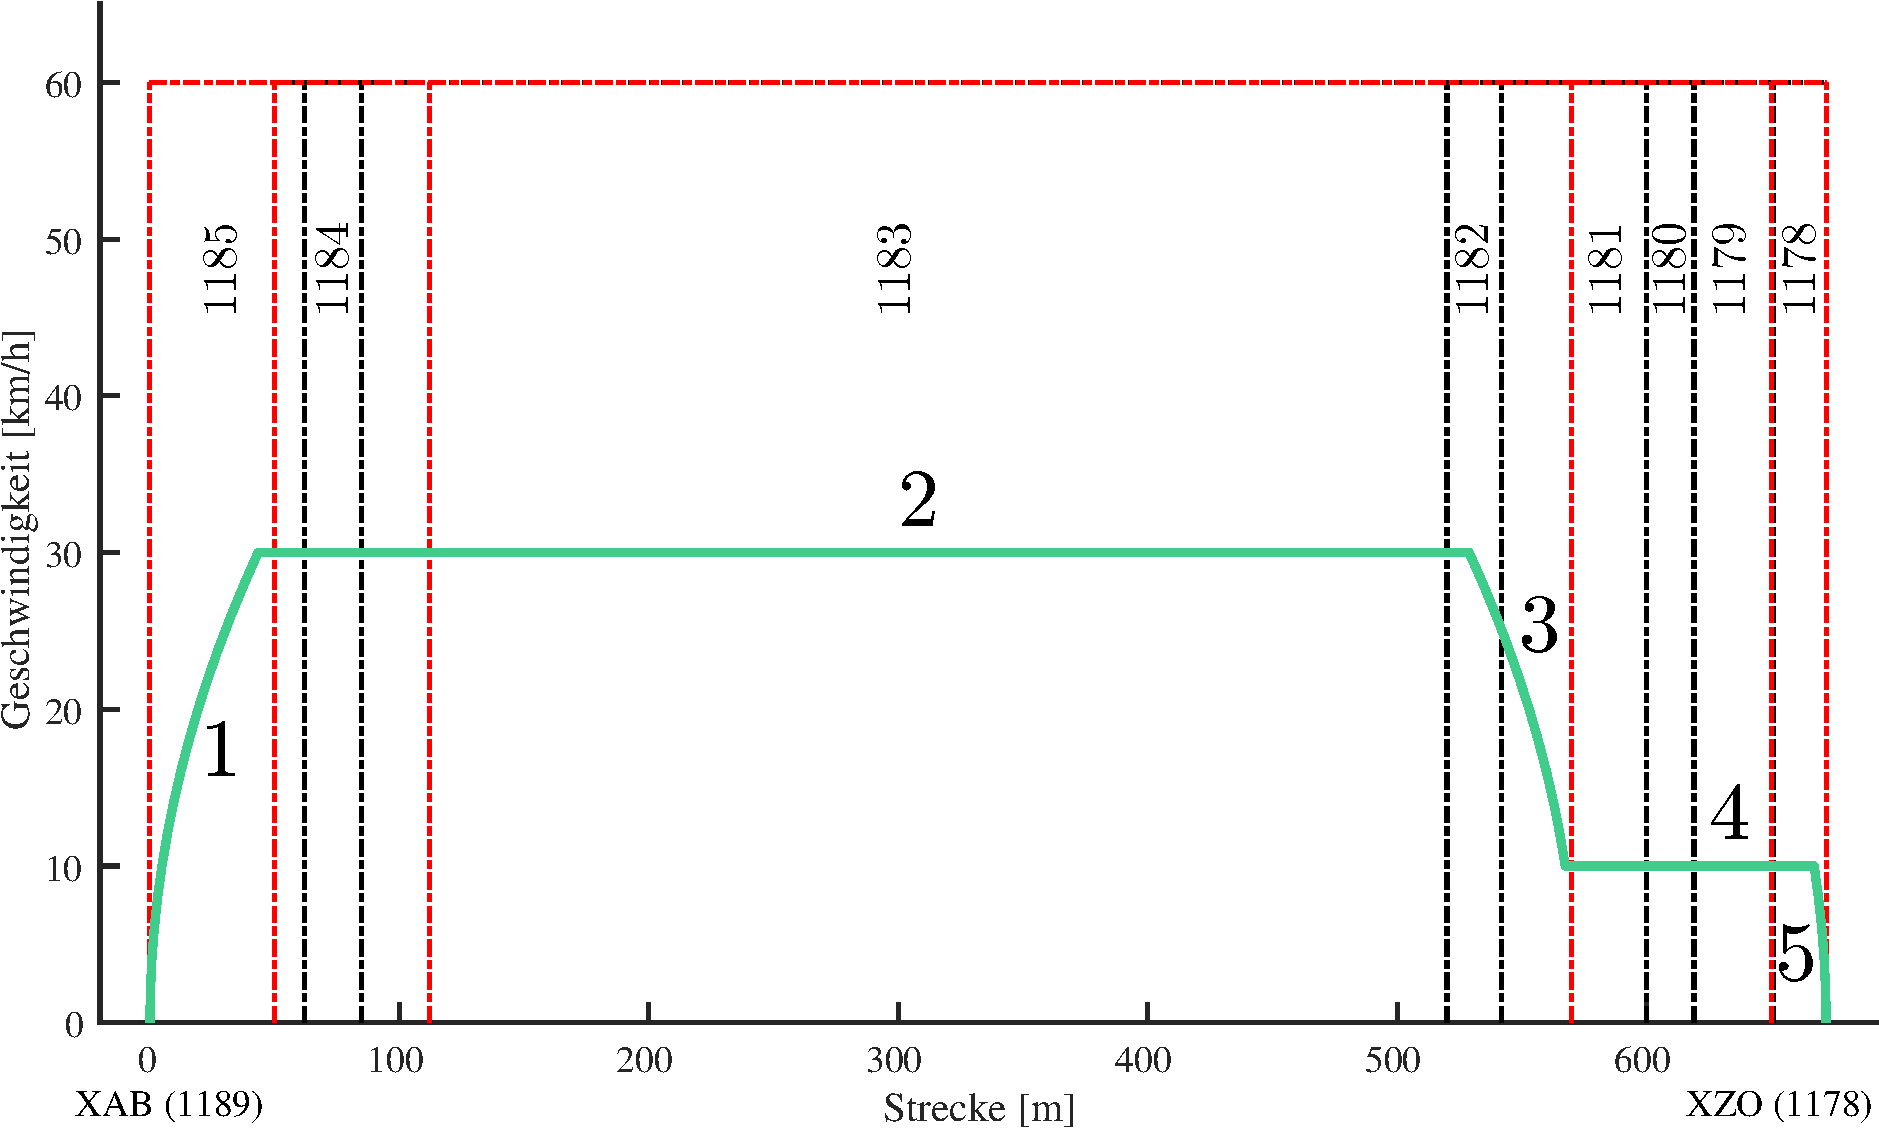
\includegraphics[width=\linewidth]{../images/matlab/it14.pdf}
\caption{\Gls{fahrtverlauf} am Beispiel von der Fahrt von XAB nach XZO}
\label{fig:it14}
\end{figure}
Durch die \textit{\$keyPoints} und die Darstellung des Fahrtverlaufs (Abbildung \ref{fig:it14}) lässt sich der Fahrtverlauf in 5 Abschnitte einteilen. Die Start- und Zielgeschwindigkeit, die Strecke und die Zeit der einzelnen Abschnitte sind in der Tabelle \ref{table:beispielebuef} aufgelistet und werden mittels der Formeln aus Kapitel \ref{formula} überprüft. Bei der Überprüfung werden die Start- und Zielgeschwindigkeiten als Grundlage genommen und untersucht, ob unter Einhaltung der gegebenen Zeit die selben Werte rauskommen.
\begin{table}
\begin{center}
\begin{threeparttable}
\renewcommand{\arraystretch}{1.2}
\begin{tabular}{c|c|c|c|c|c}
Abschnitt & \makecell{Beschleunigung/\\Verzögerung}& $v_0$ & $v_1$ & Strecke & Zeit\\ \hline
1                   &   ja (Beschleunigung)   & 0 $km/h$ & 30 $km/h$        &         43,40 $m$    & 10,42 $s$   \\ \hline
2                  &       nein& 30 $km/h$ & 30 $km/h$       &    485,43 $m$ & 58,25 $s$   \\ \hline
3                   &       ja (Verzögerung)& 30 $km/h$ & 10 $km/h$           &   38,58 $m$    & 6,94 $s$  \\ \hline
4                   &      nein & 10 $km/h$ & 10 $km/h$       &   99,76 $m$    & 35,92 $s$   \\ \hline
5                   &       ja (Verzögerung)& 10 $km/h$ & 0 $km/h$          &    4,82 $m$  & 3,47 $s$ \\ \hline
$\sum$                   &       ---& --- & ---          &    672 $m$\tnote{1}  & 115 $s$ \\ 
\end{tabular}
\begin{tablenotes}\footnotesize
    \item[1] Die Werte in der Strecken-Spalte sind auf zwei Nachkommastellen gerundet und würden durch das Aufsummieren der Strecken von Abschnitt 1 -- 5 eine Gesamtstrecke von 671,99 $m$ ergeben. Die angegebenen 672 $m$ entsprechen der Summe der Abschnitte\\1 -- 5, ohne dass die einzelnen Strecken gerundet werden.
\end{tablenotes}
\renewcommand{\arraystretch}{1}
\caption{Fahrtverlauf am Beispiel von der Fahrt von XAB nach XZO}
\label{table:beispielebuef}
\end{threeparttable}
\end{center}
\end{table}
\noindent Damit der berechnet Fahrtverlauf den Vorgaben entspricht, muss gelten:
\[t_{ges} = t_1 + t_2 + t_3 + t_4 + t_5 = 115\:s\]
%\[t_{ges} = 115s\]
\[s_{ges} = s_1 + s_2 + s_3 + s_4 + s_5 = 672\:m\]
%\[s_{ges} = 672m\]
Für die Berechnung werden die Strecken und Zeiten in gleichförmige und gleichmäßig beschleunigte Bewegungen unterteilt:
\[t_{ges} = t_{gleichförmige Bewegungen} + t_{gleichmässig Beschleunigte Bewegungen}\]
\[s_{ges} = s_{gleichförmige Bewegungen} + s_{gleichmässig Beschleunigte Bewegungen}\]
\[t_{gleichförmige Bewegungen} = t_2 + t_4\]
\[s_{gleichförmige Bewegungen} = s_2 + s_4\]
\[t_{gleichmässig Beschleunigte Bewegungen} = t_1 + t_3 + t_5\]
\[s_{gleichmässig Beschleunigte Bewegungen} = s_1 + s_3 + s_5\]
Für die gleichmäßig beschleunigten Bewegungen gilt nach den Gleichungen \ref{eq:s_v_ges} und \ref{eq:t_v_ges}:
\[t_1 = \abs{\frac{\frac{30\:km/h}{3,6}-\frac{0\:km/h}{3,6}}{0,8\:m/s^{2}}} = \frac{125}{12}\:s \approx 10,42\:s\]
\[t_3 = \abs{\frac{\frac{10\:km/h}{3,6}-\frac{30\:km/h}{3,6}}{0,8\:m/s^{2}}} = \frac{125}{18}\:s \approx 6,94\:s\]
\[t_5 = \abs{\frac{\frac{0\:km/h}{3,6}-\frac{10\:km/h}{3,6}}{0,8\:m/s^{2}}} = \frac{125}{36}\:s \approx 3,47\:s\]
\[s_1 = \frac{1}{2}\cdot\abs{\frac{{\frac{30\:km/h}{3,6}}^2-{\frac{0\:km/h}{3,6}}^2}{0,8\:m/s^{2}}} = \frac{3125}{72}\:m \approx 43,40\:m\]
\[s_3 = \frac{1}{2}\cdot\abs{\frac{{\frac{10\:km/h}{3,6}}^2-{\frac{30\:km/h}{3,6}}^2}{0,8\:m/s^{2}}} = \frac{3125}{81}\:m \approx 38,58\:m\]
\[s_5 = \frac{1}{2}\cdot\abs{\frac{{\frac{0\:km/h}{3,6}}^2-{\frac{10\:km/h}{3,6}}^2}{0,8\:m/s^{2}}} = \frac{3125}{648}\:m \approx 4,82\:m\]
Dadurch ergibt sich für die Beschleunigungen und Verzögerungen insgesamt eine\linebreak[4]Strecke von:
\[t_{gleichmässig Beschleunigte Bewegungen} = \frac{125}{6}\:s\]
\[s_{gleichmässig Beschleunigte Bewegungen} = \frac{3125}{36}\:m\]
Und für die gleichförmigen Bewegungen gilt dementsprechend:
%\[t_{gleichförmige Bewegungen} = 115s - \frac{125}{6}s\]
\[t_{gleichförmige Bewegungen} = \frac{565}{6}\:s\]
%\[s_{gleichförmige Bewegungen} = 672m - \frac{3125}{36}m\]
\[s_{gleichförmige Bewegungen} = \frac{21067}{36}\:m\]
Für die Berechnung der Strecke und Zeit von der \Gls{beharrungsfahrt} auf 30 $km/h$ gilt nach der Gleichung \ref{eq:t_1_tuning}:
\[t_{2} = \frac{s_{gleichförmige Bewegungen} - \frac{10\:km/h}{3.6} \cdot t_{gleichförmige Bewegungen}}{\frac{30\:km/h}{3.6} - \frac{10\:km/h}{3.6}}\]
\[t_{2} = \frac{\frac{21067}{36}\:m - \frac{10\:km/h}{3.6} \cdot \frac{565}{6}\:s}{\frac{30\:km/h}{3.6} - \frac{10\:km/h}{3.6}}\]
\[t_{2} = \frac{34951}{600}\:s \approx 58,25\:s\]
%\[t_{2} \approx 58,25\:s\]
Daraus folgt nach der Gleichung \ref{eq:s_v_t} für die Abschnitte 2 und 4:
\[t_{4} = \frac{7183}{200}\:s \approx 35,91\:s\]
\[s_{2} = \frac{34951}{600}\:s \cdot \frac{30\:km/h}{3,6}\]
\[s_{2} = \frac{34951}{72}\:m \approx 485,43\:m\]
%\[s_{2} \approx 485,43m\]
\[s_{4} = \frac{7183}{200}\:s \cdot \frac{10\:km/h}{3,6}\]
\[s_{4} = \frac{7183}{72}\:m \approx 99,76\:m\]
%\[s_{4} \approx 99,76m\]
In Summe ergibt das:
\[t_{ges} = \frac{125}{12}\:s + \frac{34951}{600}\:s + \frac{125}{18}\:s + \frac{7183}{200}\:s + \frac{125}{36}\:s = 115\:s\]
%\[t_{ges} = 115s\]
\[s_{ges} = \frac{3125}{72}\:m + \frac{34951}{72}\:m + \frac{3125}{81}\:m + \frac{7183}{72}\:m + \frac{3125}{648}\:m = 672\:m\]
%\[s_{ges} = 672m\]
Wie an den errechneten Werten zu erkennen ist, wurde die Mindestzeit von 20 $s$ auf einer konstanten Geschwindigkeit ($t_2$ und $t_4$) eingehalten und die Werte stimmen mit den Werten aus der Tabelle \ref{table:beispielebuef} überein.